\lstdefinelanguage{JavaScript}{
  keywords={typeof, new, true, false, catch, function, return, null, catch, switch, var, if, in, while, do, else, case, break},
  keywordstyle=\color{blue}\bfseries,
  ndkeywords={class, export, boolean, throw, implements, import, this},
  ndkeywordstyle=\color{darkgray}\bfseries,
  identifierstyle=\color{black},
  sensitive=false,
  comment=[l]{//},
  morecomment=[s]{/*}{*/},
  commentstyle=\color{purple}\ttfamily,
  stringstyle=\color{red}\ttfamily,
  morestring=[b]',
  morestring=[b]"
}

\lstset{
   language=JavaScript,
   backgroundcolor=\color{lightgray},
   extendedchars=true,
   basicstyle=\footnotesize\ttfamily,
   showstringspaces=false,
   showspaces=false,
   numbers=left,
   numberstyle=\footnotesize,
   numbersep=9pt,
   tabsize=2,
   breaklines=true,
   showtabs=false,
   captionpos=b
}


\newpage
\appendix
\section{Questionário} 
\label{form-pesquisa}

\textbf{{\large Evolução da Plataforma Mezuro}}

\begin{mdframed}
Esta é uma pesquisa relacionada à evolução do Mezuro. Direcionada aos colaboradores dessa plataforma, ela tem como objetivo extrair informações, que serão utilizadas no trabalho de conclusão de curso do aluno Vinícius Vieira, sob orientação do professor Paulo Meirelles.
\end{mdframed}

\begin{enumerate}
\item Quais os principais problemas, do ponto de vista do código e da arquitetura, do antigo Mezuro? Por que os mantenedores decidiram escrevê-lo do zero? *
\item Há aspectos do código ou da arquitetura anteriores melhores que do novo código, ou vice-versa? Quais são eles? *
\item Em relação ao código antigo, o novo código fornece (ou está previsto): *
  \begin{enumerate}
  \item As mesmas funcionalidades
  \item Menos funcionalidades
  \item Mais funcionalidades 
  \end{enumerate}
\item Em relação a questão anterior. Em caso de mais funcionalidades ou menos, quais são elas? 
\end{enumerate}

\newpage
\section{Respostas}
\label{resp-pesquisa}

{\large Respostas do Questionário}

\textbf{Respostas 1}

\begin{enumerate}
\item Quais os principais problemas, do ponto de vista do código e da arquitetura, do antigo Mezuro? Por que os mantenedores decidiram escrevê-lo do zero? *
  \begin{mdframed}
A arquitetura de plugins do Noosfero impõe limitações para a estrutura da aplicação, como rotas e também herança de controllers por exemplo. Além disso o problema com tecnologias obsoletas era sério. Ruby 1.8, além de já não receber suporte dos desenvolvedores há algum tempo, tem sérios problemas de performance corrigidos nas versões posteriores. Da mesma forma, a versão 2 do Rails é incompatível com boa parte das gemas atuais.
  \end{mdframed}
%----------------------------------------------------------------------
\item Há aspectos do código ou da arquitetura anteriores melhores que do novo código, ou vice-versa? Quais são eles? *
  \begin{mdframed}
Em suma, o novo código é melhor por que resolvemos todos os problemas da resposta anterior.
  \end{mdframed}
%---------------------------------------------------------------------
\item Em relação ao código antigo, o novo código fornece (ou está previsto): *
  \begin{enumerate}
  \item As mesmas funcionalidades
  \item Menos funcionalidades
  \item Mais funcionalidades 
  \end{enumerate}
    \begin{mdframed}
    As mesmas funcionalidades, menos funcionalidades, mais funcionalidades
    \end{mdframed}
%----------------------------------------------------------------------
\item Em relação a questão anterior. Em caso de mais funcionalidades ou menos, quais são elas? 
  \begin{mdframed}
As novas funcionalidades que temos previstas além das que já existiam estão todas descritas nas issues do github.A menos, não pretendemos fornercer uma rede social com páginas pessoais, muito menos comunidades nem suporte a temas.
  \end{mdframed}
\end{enumerate}

\textbf{Respostas 2}

\begin{enumerate}
\item Quais os principais problemas, do ponto de vista do código e da arquitetura, do antigo Mezuro? Por que os mantenedores decidiram escrevê-lo do zero? *
  \begin{mdframed}
Por antes o Mezuro ser um plugin de um software maior, nossa arquitetura era limitada ao que este software permitia fazer. Sobre o código, éramos obrigados a usar versões antigas de bibliotecas, o que fazia com que nossas soluções ficarem atrasadas com relação com o que está sendo desenvolvido no mundo do Ruby on Rails.
Por esses motivos, resolvemos escrever o código do zero, pois agora temos liberdade para mudar a arquitetura sempre que necessário e podemos usar as tecnologias mais novas.
  \end{mdframed}
%----------------------------------------------------------------------
\item Há aspectos do código ou da arquitetura anteriores melhores que do novo código, ou vice-versa? Quais são eles? *
  \begin{mdframed}
Antes o Mezuro era um plugin de um sistema maior, portanto a arquitetura era de um plugin e não de uma aplicação rails completa. No novo código, podemos desfrutar de todas as vantagens que o rails fornece. Por outro lado, antes tínhamos muita coisa já implementada que agora temos que refazer.
  \end{mdframed}
%---------------------------------------------------------------------
\item Em relação ao código antigo, o novo código fornece (ou está previsto): *
  \begin{enumerate}
  \item As mesmas funcionalidades
  \item Menos funcionalidades
  \item Mais funcionalidades 
  \end{enumerate}
    \begin{mdframed}
As mesmas funcionalidades, mais funcionalidades
    \end{mdframed}
%----------------------------------------------------------------------
\item Em relação a questão anterior. Em caso de mais funcionalidades ou menos, quais são elas? 
  \begin{mdframed}
Ampliar o escopo para analisar código Ruby, melhorar a visualização dos gráficos e dos resultados, notificação de alerta quando uma métrica atingir certo valor considerado ruim, entre outras.
  \end{mdframed}
\end{enumerate}

\newpage
\section{Questionário PSSUQ - Satisfação de Usabilidade Plataforma Mezuro}
\label{questionario-pssuq}
\graphicspath{{figuras/}}
\begin{figure}[H]
\centering
\includegraphics[width=1.0\textwidth]{PSSUQ1}
\label{pssuq1}
\end{figure}

\graphicspath{{figuras/}}
\begin{figure}[H]
\centering
\includegraphics[width=1.0\textwidth]{PSSUQ2}
\label{pssuq2}
\end{figure}

\graphicspath{{figuras/}}
\begin{figure}[H]
\centering
\includegraphics[width=1.0\textwidth]{PSSUQ3}
\label{pssuq3}
\end{figure}

\newpage
\section{Proposta de práticas de usabilidade ágil para a comunidade de software livre}\footnote{Seção retirada da dissertação de mestrado Ana Paula Oliveira dos Santos}
\label{ap-praticas-usabilidade}

\textbf{Identificar necessidades para design centrado em humano}

\textbf{Equipe-Núcleo como Donos do Produto}

Contexto: Equipe de desenvolvimento de software livre composta por desenvolvedores e que não possui especialistas em usabilidade ou UX como membros. Contudo, a equipe-núcleo do projeto percebe a necessidade de compreender melhor os requisitos de negócios e de usabilidade, levando em consideração a visão de clientes e usuários típicos.
Problema: Integrar requisitos de negócio com requisitos de usabilidade em um ambiente que não possui especialistas em usabilidade. Principais forças envolvidas:
\begin{itemize}
\item Força 1: Necessidade de levantamento de requisitos de negócios com clientes e requisitos de usabilidade com usuários típicos, de modo a integrá-los para o desenvolvimento do sistema.
\item Força 2: Não existe garantia de que especialistas em usabilidade ou UX participarão voluntariamente do projeto e/ou não é possível contratá-los. Também não é possível garantir que desenvolvedores voluntários queiram participar dessas atividades.
\end{itemize}
Solução: Uma adaptação da prática Especialistas em UX como Donos do Produto, da comunidade de métodos ágeis, na qual a equipe-núcleo de um projeto de software livre assumiria o papel de Proprietários do Produto, que levam em consideração a usabilidade do sistema. Dessa forma, podem controlar as contribuições para o projeto, com a visão das necessidades de usuários típicos e clientes.

%
\textbf{Caminhos Completos}

Contexto: Equipe de desenvolvimento de software livre composta por desenvolvedores e que não possui especialistas em usabilidade ou UX como membros. Contudo, a equipe-núcleo do projeto precisa empregar práticas de usabilidade durante o desenvolvimento do sistema.
Problema: Realizar práticas de usabilidade em projetos de software livre que não possuem especialistas em usabilidade ou UX. Principais forças envolvidas:
\begin{itemize}
\item Força 1: Necessidade de realizar práticas de usabilidade para pesquisa de usuários, levanta- mento de requisitos e metas de usabilidade, definição de design e avaliações com usuários e clientes.
\item Força 2: Não existe garantia de que especialistas em usabilidade ou UX participarão voluntariamente do projeto e/ou não é possível contratá-los.
\item Força 3: Desenvolvimento distribuído e participação esporádica de membros.
\end{itemize}
Solução: Em vez de caminhos paralelos entre equipe de desenvolvimento e de UX, como ocorre na prática Caminhos paralelos da comunidade de métodos ágeis, a equipe de desenvolvimento executa o ciclo completo de DCU para um conjunto específico de funcionalidades, utilizando-se de Pouco design antecipado ou Pouco design antecipado e distribuído para coletar informações. A prática pode ser executada apenas pela equipe-núcleo do projeto ou mesmo com a participação dos demais contribuidores que desejem participar.

%
\textbf{Especialista-generalista}

Contexto: Equipes de desenvolvimento de software livre, que não possuem especialistas em usabilidade ou UX como membros do time, compostas por desenvolvedores que desejam desenvolver sistemas com melhor usabilidade para usuários típicos.
Problema: Ausência de especialistas em usabilidade ou UX na equipe de desenvolvimento do projeto. Principais forças envolvidas:
\begin{itemize}
\item Força 1: Não existe garantia de que especialistas em usabilidade ou UX participarão voluntariamente do projeto e/ou não é possível contratá-los.
\item Força 2: Desenvolvimento distribuído e participação esporádica de membros.
\end{itemize}
Solução: Os desenvolvedores da equipe-núcleo do projeto aplicam práticas de usabilidade para entender quem são os usuários típicos do sistema, quais são as suas necessidades e em que contexto o sistema seria utilizado, de modo a incluir essas considerações nos requisitos da aplicação. As pesquisas têm baixa granularidade, ou seja, realiza-se apenas o necessário para o entendimento das funcionalidades da próxima iteração. Os requisitos podem ser definidos por meio da escrita de cartões de histórias de usuários, que são validados com o cliente conforme ocorre em comunidades de métodos ágeis. A documentação detalhada dos requisitos pode ser encontrada nos testes de aceitação, que podem ser acessados por qualquer desenvolvedor do sistema, conforme a prática Testes de aceitação de comunidades de métodos ágeis, o que mantém um relatório atualizado das funcionalidades do sistema que atendem ao comportamento esperado. As metas de usabilidade do sistema também podem ser descritas por meio da proposta de prática Definir metas de usabilidade automáticas.


%
\textbf{Especificar contexto de uso}

\textbf{Pouco design antecipado e distribuído}

Contexto: Equipe de desenvolvimento de software livre composta por desenvolvedores e que não possui especialistas em usabilidade ou UX como membros. Membros da equipe-núcleo do projeto e contribuidores encontram-se distribuídos em diversas localidades. Contudo, existe a necessidade de realização de pesquisas presenciais com usuários típicos para melhor compreensão do contexto de uso do sistema.
Problema: Utilizar práticas de usabilidade, em ambiente de desenvolvimento de software livre, para especificar contexto de uso de um sistema, onde membros da equipe estão dispersos em vários locais diferentes. Principais forças envolvidas:
\begin{itemize}
\item Força 1: Distância física entre membros de uma comunidade de desenvolvimento de software livre.
\item Força 2: Necessidade de realização de pesquisas de usabilidade para definição de perfil de usuários típicos e o contexto de uso do sistema.
\item Força 3: Possibilitar a participação de voluntários de diversas culturas.
\end{itemize}
Solução: Equipe-núcleo do projeto é responsável por definir quais são as práticas de usabilidade a serem utilizadas para especificação do contexto de uso de um sistema e também por realizar as práticas presenciais na sua cidade. Membros da equipe, que se encontram dispersos em locais distintos, poderiam aplicar a mesma prática em sua localidade, de modo a obter feedback de usuários com culturas diferentes; por exemplo, replicando testes, sessões de grupos focais ou entrevistas presenciais, em sua região ou país. Desse modo, possibilita-se a obtenção da percepção cultural de vários locais distintos, de modo a explorar o contexto de projetos abertos, no qual podem existir desenvolvedores, usuários, membros da equipe-núcleo e contribuidores em diversas localidades.


%
\textbf{Especificar requisitos}

\textbf{Definir metas de usabilidade automáticas}

Contexto: Desenvolvimento aberto, distribuído e colaborativo, onde desenvolvedores podem entrar e sair do projeto durante o processo de desenvolvimento. Também não existe uma equipe de usabilidade trabalhando em conjunto com a equipe de desenvolvimento.
Problema: Definir metas de usabilidade de modo que todos os desenvolvedores que contribuam com um projeto aberto possam conhecer as metas definidas. Principais forças envolvidas:
\begin{itemize}
\item Força 1: Necessidade de definição de metas de usabilidade que atendam às necessidades de usuários típicos.
\item Força 2: Possibilitar que todos os desenvolvedores tenham contato diário com as metas de usabilidade definidas
\item Força 3: Desenvolvimento distribuído e participação esporádica de membros.
\item Força 4: Manter documentação atualizada das metas de usabilidade tratadas pelo sistema.
\end{itemize}
Solução: Escrita de testes de aceitação automáticos baseados em Behaviour Driven Development
(BDD) para definição de metas de usabilidade. Para o contexto de desenvolvimento livre, seria mais eficiente escrever as metas de usabilidade diretamente no ambiente de desenvolvimento do que em documentos separados, que correm o risco de não serem lidos. Sendo assim, conforme grupos de funcionalidades são selecionados para desenvolvimento, descreve-se as metas de usabilidade que precisam ser cumpridas para essas funcionalidades. Membros da equipe-núcleo do projeto podem escrever testes de aceitação automáticos, envolvendo usuários típicos e/ou clientes, o que possibilita documentar o comportamento esperado para a funcionalidade, e também gerar um relatório do funcionamento do sistema, exibindo quais funcionalidades e quais cenários são implementados de acordo com as necessidades dos usuários reais.


%
\textbf{Avaliar designs}

\textbf{RITE (Rapid Iterative Testing and Evaluation)  para desenvolvedores de software livre}

Contexto: Equipes de desenvolvimento de software livre que não possuem especialistas em usabilidade ou UX como membros do time, mas que tem a necessidade de realizar testes de usabilidade com usuários típicos do sistema de modo a desenvolver sistemas com melhor usabilidade.
Problema: Possibilitar a identificação e correção de problemas de usabilidade no menor tempo possível durante o desenvolvimento de software livre. Principais forças envolvidas:
\begin{itemize}
\item Força 1: Diminuir a distância entre a identificação e a correção de problemas de usabilidade encontrados em testes com usuários.
\item Força 2: Não existe garantia de que especialistas em usabilidade ou UX participarão voluntariamente do projeto e/ou não é possível contratá-los.
\end{itemize}
Solução: O método RITE pode ser aplicado por membros da equipe-núcleo do projeto, não sendo
necessário utilizar laboratórios de usabilidade com a aplicação de testes formais. Os desenvolvedores da equipe-núcleo podem observar os usuários utilizando um pequeno conjunto de funcionalidades do sistema e solicitar que falem em voz alta o que estão pensando, enquanto o utilizam (Protocolo Pensando em voz alta). Não seria necessária a criação de relatórios e análises de vídeo dos testes, pois os desenvolvedores que estarão envolvidos na correção dos problemas encontrados podem participar do teste como moderadores ou observadores, de modo que possam obter o conhecimento das melhorias necessárias que precisam ser implementadas. Para documentar problemas referentes a um comportamento esperado do sistema, os testes de aceitação automáticos, utilizados pela comunidade de métodos ágeis, podem servir como forma de documentação, como também, para verificar se o sistema está realizando a tarefa do modo que se espera. Nesse caso, o relatório de teste de usabilidade seria substituído por testes de aceitação automáticos. A criação dos testes de aceitação, nesse caso, seria feita pelos próprios desenvolvedores que participaram do teste e conhecem o problema a ser resolvido. Um breve brainstorming após a sessão de teste serviria para consolidar as impressões dos membros da equipe envolvidos, possibilitando definir como os problemas serão corrigidos. A correção dos problemas encontrados seria realizada na sequência da realização do teste. Dessa forma, os testes de aceitação serviriam para registrar como corrigir um problema de usabilidade, detectado no teste com usuários típicos, para um determinado cenário de uso do sistema.

\newpage
\section{Revisão Sistemática: Técnicas de usabilidade em projetos ágeis aplicadas no desenvolvimento de software livre}\footnote{Seção retirada da revisão sistemática realizada no processo de desenvolvimento do trabalho}
\label{revisao-tecnicas-usabilidade}

O objetivo desta revisão sistemática é analisar relatos de experiência da abordagem de
usabilidade nas comunidades ágeis que possam ser aplicadas na comunidade de software
livre, com o propósito de identificar e analisar técnicas de usabilidade, com relação à
forma que a usabilidade é abordada em projetos ágeis, do ponto de vista de organizações
que implementam técnicas de usabilidade no processo de desenvolvimento envolvidas nas
iniciativas e no contexto de projetos e estudos de caso reais.

Questão de pesquisa definida para alcançar o objetivo descrito:

1. Quais técnicas de usabilidade são abordadas nas comunidades ágeis e software
livre?

Em relação ao escopo da pesquisa, os critérios adotados para selecionar as fontes
de busca foram: bases com renome e difundidas na área de TI; que grande quantidade
de material publicado e engenhos de busca intuitivos para filtrar os resultados; e possuir
relação com o tema a ser pesquisado. Outro ponto levantado foi selecionar bases que
pudessem evidenciar o cenário das universidades brasileiras em relação ao tema.

Foram selecionadas as bases de busca Google Academic e Springer Link que possuem máquinas de busca com bom funcionamento e abrangência, além das bibliotecas digitais da UnB e USP.

Foram utilizados os termos em inglês e uma tradução em português. Uma primeira
 string de busca foi formulada, porém por mais que abordasse aspectos da hipótese continha termos muito genéricos como palavras chave (Usability, Free Software e Agile Method). Obteve assim resultados demasiados, chegando a encontrar mais de mil artigos em apenas uma única base, dificultando a filtragem e busca de artigos adequados e relevantes ao tema.

A fim de obter um resultado mais expressivo em relação a questão levantada, em
 um domínio mais específico criou-se uma nova String: ((”technical usability” or ”usability practices” or ”interaction design” and usability) and (“free software” or ”open source”)
 and “agile software development”) com uma variação de sintaxe para se adequar a todas as bases selecionadas: ((”technical usability” OR ”usability practices” OR ”interaction
 design” AND usability) AND (“free software” OR ”open source”) AND “agile software
 development”). Os termos da expressão relacionados a usabilidade estão voltados para implementação, aplicação e parte prática. Os outros termos restringem os resultados para as abordagens das comunidades e projetos ágeis e de software livre.

A seleção dos artigos foi realizada em 5 etapas:
1. Seleção e catalogação preliminar dos artigos coletadas nas fontes a partir da expressão de busca;
2. Filtro de seleção dos artigos relevantes - 1, verificar data de publicação aplicando
o critério de seleção ”CS1 – ter sido publicado entre 2007 até 2013”;
3. Filtro de seleção dos artigos relevantes - 2, por meio da ferramenta de busca filtrar
resultados por relevância (critérios definidos pela base de busca) e selecionar os
20 primeiros da lista;
4. Filtro de seleção dos artigos relevantes - 3, por meio de análise do resumo (abstract) e aplicando o critério de seleção ”CS2 - possuir informações sobre técnicas de usabilidade na comunidade ágil ou software livre”;
5. Filtro de seleção dos artigos relevantes - 4, por meio da leitura completa dos artigos e aplicando os critérios de seleção ”CS3- possuir evidência de técnicas que
 foram praticadas, utilizadas, discutidas dentro de um projeto ágil ou de software livre”.

Para os artigos considerados relevantes, os seguintes dados foram extraídos: dados do artigo (título, autor(es), data da publicação, fonte de publicação), resumo do artigo, listagem de como as técnicas de usabilidade foram adotadas e quais técnicas de usabilidade foram abordadas em projetos ágeis ou de software livre.

Os dados coletados nos artigos selecionados foram analisados quantitativa e qualitativamente. A análise qualitativa se deu através de um mapeamento das técnicas encontradas e como elas interagiram. A análise quantitativa resultou em uma lista das técnicas que podem ser aplicadas pelas comunidades de software livre.

\textbf{Resultado da Revisão sistemática}

Com o estabelecimento do protocolo da revisão sistemática, a pesquisa foi executada em
Outubro de 2013. Na primeira etapa de seleção dos artigos, a expressão de busca foi
executada nas máquinas de buscas Google Academic e Springer Link e verificada nos arquivos das bibliotecas digitais das universidades USP e UnB. No Google Academic,
165 artigos foram obtidas e no Springer Link foram retornadas 55, sendo 19 comuns com
o Google Academic. Nas universidades nacionais, a USP retornou 6 resultados e na UnB
nenhum artigo que atendesse à expressão de busca foi encontrada.

Na primeira etapa de seleção dos artigos, o critério de seleção CS1, foi aplicado
filtrando os artigos de entre o período de 2007 até 2013. No Google Academic, 118
resultados foram obtidos, porém 12 destes eram livros ficando 106 artigos e no Springer
Link foram retornadas 52, sendo 16 comuns com o Google Academic e na USP 3 dos
resultados eram apenas links sem referência a artigos, restando assim 3 artigos.

Na segunda etapa de seleção dos artigos, os artigos foram filtradas de acordo com
a relevância e foram selecionados os 20 primeiros resultando em um total de 43 artigos
selecionados.

Na terceira etapa de seleção dos artigos, o resumo (abstract) de cada artigo foi lido.
Seguindo o critério de seleção CS2, os artigos que não apresentavam o resumo (abstract)
via engenho de busca foram descartadas automaticamente, assim selecionando dez artigos
conforme apresentado na Figura \ref{fig-revisao1}.

\graphicspath{{figuras/}}
\begin{figure}[htpb]
\centering
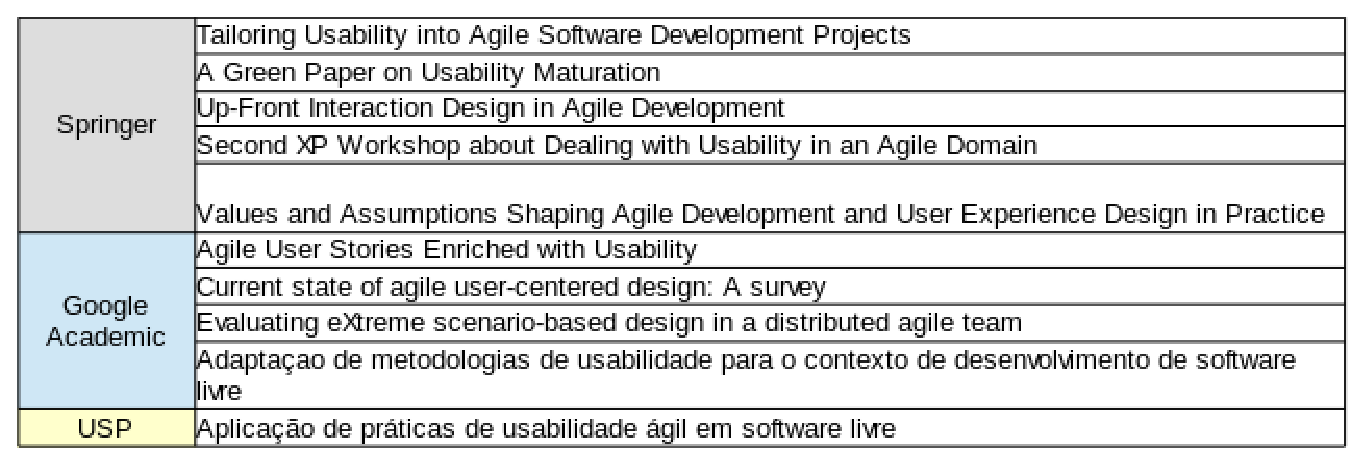
\includegraphics[width=0.8\textwidth]{tabela2}
\caption{Terceira etapa de seleção dos artigos}
\label{fig-revisao1}
\end{figure}

Durante a obtenção dos artigos 3 foram eliminados devido a falta de acesso e um
por não conter seu desenvolvimento apenas breve descrição e resumo. Na quarta etapa
de seleção dos artigos com os 7 artigos remanescentes, foi realizada a leitura completa
dos artigos aplicando o critério de seleção CS3 para verificar a adequação junto a questão
levantada.

Os artigos selecionados levaram a seleção de 8 técnicas de usabilidade utilizadas na comunidade ágil que podem ser aplicadas na comunidade de software livre. Essas técnicas
foram propostas visando os princípios e práticas ágeis e algumas validadas em projetos
ágeis, elas podem ser agrupas em 3 tipos, histórias de usabilidade, design centrado no
usuário e outros.



\newpage
\section{Código-Fonte}
\label{source-code-appendix}

\subsection{Feature Repositórios}
\subsubsection{\textit{Controller}}
\begin{lstlisting}[language=Ruby]
include OwnershipAuthentication

class RepositoriesController < ApplicationController
  before_action :authenticate_user!, except: [:show, :state]
  before_action :project_owner?, only: [:new, :create]
  before_action :repository_owner?, only: [:edit, :update, :destroy, :process_repository]
  before_action :set_repository, only: [:show, :edit, :update, :destroy, :state, :process_repository]

  # GET /projects/1/repositories/1
  # GET /projects/1/repositories/1.json
  # GET /projects/1/repositories/1/modules/1
  # GET /projects/1/repositories/1/modules/1.json
  def show
    set_configuration
  end

  # GET projects/1/repositories/new
  def new
    @project_id = params[:project_id]
    @repository = Repository.new
    @repository_types = Repository.repository_types
  end

  # GET /repositories/1/edit
  def edit
    @project_id = params[:project_id]
    @repository_types = Repository.repository_types
  end

  # POST /projects/1/repositories
  # POST /projects/1/repositories.json
  def create
    @repository = Repository.new(repository_params)
    @repository.project_id = params[:project_id]
    respond_to do |format|
      create_and_redir(format)
    end
  end

  # PUT /projects/1/repositories/1
  # PUT /projects/1/repositories/1.json
  def update
    respond_to do |format|
      if @repository.update(repository_params)
        format.html { redirect_to(project_repository_path(params[:project_id], @repository.id), notice: 'Repository was successfully updated.') }
        format.json { head :no_content }
      else
        failed_action(format, 'edit')
      end
    end
  end

  # DELETE /projects/1/repositories/1
  # DELETE /projects/1/repositories/1.json
  def destroy
    @repository.destroy
    respond_to do |format|
      format.html { redirect_to project_path(params[:project_id]) }
      format.json { head :no_content }
    end
  end

  # POST /projects/1/repositories/1/state
  def state
    if params[:last_state] != 'READY'
      if params[:day].nil?
        @processing = @repository.last_processing
      else
        year, month, day = params[:year], params[:month], params[:day]
        @processing = Processing.processing_with_date_of(@repository.id, "#{year}-#{month}-#{day}")
      end

      respond_to do |format|
        if @processing.nil?
          format.js { render action: 'unprocessed' }
        elsif @processing.state == 'READY'
          format.js { render action: 'load_ready_processing' }
        else
          format.js { render action: 'reload_processing' }
        end
      end
    else
      head :ok, :content_type => 'text/html' # Just don't do anything
    end
  end

  # GET /projects/1/repositories/1/process
  def process_repository
    @repository.process
    set_configuration
    respond_to do |format|
      format.html { redirect_to project_repository_path(@repository.project_id, @repository.id) }
    end
  end

private
  # Duplicated code on create and update actions extracted here
  def failed_action(format, destiny_action)
    @project_id = params[:project_id]
    @repository_types = Repository.repository_types

    format.html { render action: destiny_action }
    format.json { render json: @repository.errors, status: :unprocessable_entity }
  end

  # Use callbacks to share common setup or constraints between actions.
  def set_repository
    @repository = Repository.find(params[:id].to_i)
  end

  def set_configuration
    @configuration = MezuroConfiguration.find(@repository.configuration_id)
  end

  # Never trust parameters from the scary internet, only allow the white list through.
  def repository_params
    params[:repository]
  end

  # Code extracted from create action
  def create_and_redir(format)
    if @repository.save
      format.html { redirect_to project_repository_process_path(@repository.project_id, @repository.id), notice: 'Repository was successfully created.' }
    else
      failed_action(format, 'new')
    end
  end

end
\end{lstlisting}

%\subsubsection{\textit{Model}}
%ass Repository < KalibroGatekeeperClient::Entities::Repository
%	include KalibroRecord
%
%  validates :name, presence: true, kalibro_uniqueness: true
%  validates :address, presence: true
%
%  def last_processing
%    if Processing.has_processing(@id)
%      Processing.processing_of(@id)
%    else
%      nil
%    end
%  end
%end
%
%\end{lstlisting}
%\begin{lstlisting}[language=Ruby]
%class Repository < KalibroGatekeeperClient::Entities::Repository
%	include KalibroRecord
%
%  validates :name, presence: true, kalibro_uniqueness: true
%  validates :address, presence: true
%
%  def last_processing
%    if Processing.has_processing(@id)
%      Processing.processing_of(@id)
%    else
%      nil
%    end
%  end
%end
%\end{lstlisting}

\subsection{Feature Configuration}
\subsubsection{\textit{Controller}}
\begin{lstlisting}[language=Ruby]
class MetricConfigurationsController < BaseMetricConfigurationsController
  def choose_metric
    @mezuro_configuration_id = params[:mezuro_configuration_id].to_i
    @metric_configuration_id = params[:metric_configuration_id].to_i
    @base_tools = KalibroGatekeeperClient::Entities::BaseTool.all
    @exist_metric = params[:exist_metric]
  end

  def new
    super
    @metric_configuration = MetricConfiguration.new
    @metric_configuration.configuration_id = params[:mezuro_configuration_id].to_i
    @metric_configuration.base_tool_name = params[:base_tool_name]
  end

  def create
    @configuration_metrics = params[:configuration_metrics_names]
    
    @configuration_metrics.each do |configuration_metric|
      code = automatic_code configuration_metric
      @metric_configuration = MetricConfiguration.new
      @metric_configuration.configuration_id = params[:mezuro_configuration_id].to_i
      @metric_configuration.base_tool_name = "Analizo"
      @metric_configuration.metric = KalibroGatekeeperClient::Entities::BaseTool.find_by_name("Analizo").metric(configuration_metric.to_s)
      @metric_configuration.code = code.to_s
      @metric_configuration.weight = "0"
      @metric_configuration.aggregation_form = "AVERAGE"
      @metric_configuration.reading_group_id = 1
      @metric_configuration.save
    end
    respond_to do |format|
      create_and_redir(format)
    end    
  end

  def automatic_code(metric_name)
    array = metric_name.split(" ", 3);
    automatic_code = ""
    array.each do |metric_word|
      automatic_code = automatic_code << metric_word[0...2]
    end
    automatic_code
  end

  def edit
    #FIXME: set the configuration id just once!
    @mezuro_configuration_id = params[:mezuro_configuration_id]
    @metric_configuration.configuration_id = @mezuro_configuration_id
  end

  def update
    puts '=' * 100
    puts 'I reached the action controller!'
    respond_to do |format|
      @metric_configuration.configuration_id = params[:mezuro_configuration_id]
      if @metric_configuration.update(metric_configuration_params)
        format.html { redirect_to(mezuro_configuration_path(@metric_configuration.configuration_id), notice: 'Metric Configuration was successfully updated.') }
        format.json { head :no_content }
      else
        failed_action(format, 'edit')
      end
    end
  end

  def destroy
    @metric_configuration.destroy
    respond_to do |format|
      format.html { redirect_to mezuro_configuration_path(params[:mezuro_configuration_id]) }
      format.json { head :no_content }
    end
  end

  protected

  def metric_configuration
    @metric_configuration
  end

  def update_metric_configuration (new_metric_configuration)
    @metric_configuration = new_metric_configuration
  end

  private

  # Duplicated code on create and update actions extracted here
  def failed_action(format, destiny_action)
    @mezuro_configuration_id = params[:mezuro_configuration_id]

    format.html { render action: destiny_action }
    format.json { render json: @metric_configuration.errors, status: :unprocessable_entity }
  end

  #Code extracted from create action
  def create_and_redir(format)
    if @metric_configuration.save
      format.html { redirect_to mezuro_configuration_path(@metric_configuration.configuration_id), notice: 'Metric Configuration was successfully created.' }
    else
      failed_action(format, 'new')
    end
  end
end

\end{lstlisting}

%\subsubsection{\textit{Model}}
%\begin{lstlisting}[language=Ruby]
%require "validators/kalibro_uniqueness_validator.rb"
%
%class MezuroConfiguration < KalibroGatekeeperClient::Entities::Configuration
%  include KalibroRecord
%
%  attr_accessor :name
%  validates :name, presence: true, kalibro_uniqueness: true
%
%  def metric_configurations
%    MetricConfiguration.metric_configurations_of(self.id)
%  end
%end
%\end{lstlisting}


\begin{lstlisting}
include OwnershipAuthentication

class MezuroConfigurationsController < ApplicationController
  before_action :authenticate_user!, except: [:index, :show]
  before_action :mezuro_configuration_owner?, only: [:edit, :update, :destroy]

  # GET /mezuro_configurations/new
  def new
    @mezuro_configuration = MezuroConfiguration.new
  end

  # GET /mezuro_configurations
  # GET /mezuro_configurations.json
  def index
    @mezuro_configurations = MezuroConfiguration.all
  end

  # POST /mezuro_configurations
  # POST /mezuro_configurations.json
  def create
    @mezuro_configuration = MezuroConfiguration.new(mezuro_configuration_params)
    respond_to do |format|
      create_and_redir(format)
    end
  end

  # GET /mezuro_configurations/1
  # GET /mezuro_configurations/1.json
  def show
    set_mezuro_configuration
    @mezuro_configuration_metric_configurations = @mezuro_configuration.metric_configurations
  end

  # GET /mezuro_configurations/1/edit
  # GET /mezuro_configurations/1/edit.json
  def edit
    set_mezuro_configuration
  end


  def update
    set_mezuro_configuration
    if @mezuro_configuration.update(mezuro_configuration_params)
      redirect_to(mezuro_configuration_path(@mezuro_configuration.id))
    else
      render "edit"
    end
  end

  # DELETE /mezuro_configurations/1
  # DELETE /mezuro_configurations/1.json
  def destroy
    set_mezuro_configuration
    current_user.mezuro_configuration_ownerships.find_by_mezuro_configuration_id(@mezuro_configuration.id).destroy
    @mezuro_configuration.destroy
    respond_to do |format|
      format.html { redirect_to mezuro_configurations_url }
      format.json { head :no_content }
    end
  end

  private
  # Use callbacks to share common setup or constraints between actions.
  def set_mezuro_configuration
    @mezuro_configuration = MezuroConfiguration.find(params[:id])
  end

  # Never trust parameters from the scary internet, only allow the white list through.
  def mezuro_configuration_params
    params[:mezuro_configuration]
  end

  # Extracted code from create action
  def create_and_redir(format)
    if @mezuro_configuration.save
      current_user.mezuro_configuration_ownerships.create mezuro_configuration_id: @mezuro_configuration.id

      format.html { redirect_to mezuro_configuration_path(@mezuro_configuration.id), notice: 'mezuro configuration was successfully created.' }
      format.json { render action: 'show', status: :created, location: @mezuro_configuration }
    else
      format.html { render action: 'new' }
      format.json { render json: @mezuro_configuration.errors, status: :unprocessable_entity }
    end
  end
end

\end{lstlisting}

\subsection{Gráfico Radar}
\label{radar-chart-code}
Nesta subseção se encontra o código-fonte referente a aplicação da técnica de visualização do Radar. O script abaixo encontra-se na \textit{view} \textit{show.html} da entidade \textit{Repository}, a qual é responsável pela abertura do \textit{modal}, que é a estrutura visual gerada, por cima da \textit{view} principal, para apresentar o gráfico.

\begin{lstlisting}

<script type="text/javascript">

$('#my-modal').on('show', function () {

    $(this).find('.modal-body').css({
      width:'auto',
      height:'auto', 
      'max-height':'100%'});
});

var w = 500,
h = 500;

var colorscale = d3.scale.category10();

//Data
var myData = new Array([]);

d3.tsv("/data.tsv", type, function(error, data) {
  
  for (var i = 0; i < data.length; i++) { 
    var map = {};
    map["axis"] = data[i].axis;
    map["value"] = data[i].value;   
    myData[0][i] = map;
  }
  console.log(myData[0]);

  //Call function to draw the Radar chart
  RadarChart.draw("#chart", myData, mycfg);
});

function type(d) {
  d.value = +d.value; // coerce to number
  return d;
}

//Options for the Radar chart, other than default
var mycfg = {
  w: w,
  h: h,
  maxValue: 150,
  levels: 5,
  ExtraWidthX: 200
}

</script>

\end{lstlisting}

O código abaixo é referente a estrutura que contem o gráfico, o chamado \textit{modal}.

\begin{lstlisting}
<div class="modal hide fade" id="my-modal" title="Radar Chart">
  <div class="modal-header">
    <button aria-hidden="true" class="close" data-dismiss="modal" type="button">x</button>
    <h3 id="myModalLabel">Visualization</h3>
  </div>
  <div class="modal-body" id="chart">
    <h4>Radar Chart</h4>
  </div>
  <div class="modal-footer">
    <button aria-hidden="true" class="btn" data-dismiss="modal">Close</button>
  </div>
</div>
\end{lstlisting}

\begin{lstlisting}
<%= link_to "Visualize", "#my-modal", :class => "btn", "data-toggle" => "modal" %>
\end{lstlisting}

\subsection{CSS formwithtooltip}
\label{css-form}

\begin{lstlisting}
.form-table {
  margin: 0 !important;
  background: #fff;
  -webkit-box-shadow: 0 1px 2px rgba(0, 0, 0, 0.075);
  box-shadow: 0 1px 2px rgba(0, 0, 0, 0.075);
}

.form-row {
  float: left;
  width: 100%;
  border-bottom: 1px solid #f2f2f2;
  border-top: 1px solid #e3e3e3;
  display: inline-flex;
}

.field-container {
  position: relative;
  float: left;
  width: 653px;
  padding: 20px;
}

.help-container {
  float: left;
  width: 400px;
  padding: 20px;
  background: #f5f5f5;
  border-left: 1px solid #e3e3e3;
  border-right: 1px solid #e3e3e3;
}

.text-field {
  width: 95% !important;
  margin: 0;
  background: #f9f9f9;
}

.text-area {
  width: 95% !important;
  margin: 0;
}

.field-container select {
  width: 99% !important;
  margin: 0;
}
\end{lstlisting}
